\section{状态表示}
\label{sec:ivp-state}

定义~\ref{def:ivp-ivp}只含一阶导数，而力学里的方程通常是二阶的。此刻的哪些量足以决定未来？回答这个问题，就能把高阶方程放进同一个框架，也能把时间、输入与状态分开。

\paragraph{摆只知道角度够不够}
图~\ref{fig:ivp-pendulum-diagram}是一个单摆。设摆长为$\ell$，$y(t)$是摆杆偏离竖直方向的角度（弧度），重力加速度记作$\gamma$。忽略阻力，重力沿圆弧切向的分量是$-\gamma\sin y$，切向加速度是$\ell\ddot{y}$，Newton第二定律给出
\begin{equation}
 \ddot{y}=-\kappa\sin y,\qquad\kappa=\frac{\gamma}{\ell}.
 \label{eq:ivp-pendulum}
\end{equation}
以下取时间单位使$\kappa=1$。

\begin{BookInlineFigure}
 \centering
 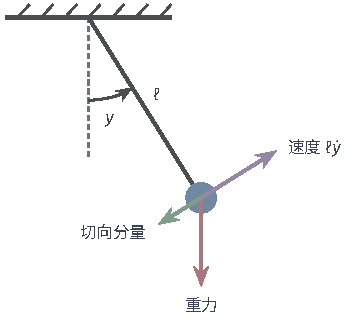
\includegraphics[width=60mm]{figures/06-differential-equations/01-ordinary-differential-equations/tikz/ivp-pendulum-diagram/figure.pdf}
 \caption{单摆的受力。$y$是摆杆与竖直方向的夹角，$\ell$是摆长。红色箭头是重力，绿色箭头是它沿圆弧切向的分量，紫色箭头是摆球的速度，大小为$\ell\lvert\dot{y}\rvert$。}
 \label{fig:ivp-pendulum-diagram}
\end{BookInlineFigure}

式~\eqref{eq:ivp-pendulum}给出的是加速度。只知道此刻的角度，能算出加速度，却算不出角度的变化率。同样在$y=1$的位置，摆球可能静止，也可能正在向上或向下运动，接下来的走向完全不同。图~\ref{fig:ivp-pendulum-state}(a)的三条曲线都从$y=1$出发，初始角速度分别是$0$、$1$和$-1$。

由此得到选择状态的原则：\term{状态}（state）是此刻的一组量，有了它和方程，下一瞬间的变化就完全确定，不需要回头查看历史。单摆需要角度和角速度两个量。令
\[
 x_1=y,\qquad x_2=\dot{y},
\]
则$\dot{x}_1=x_2$，而由式~\eqref{eq:ivp-pendulum}有$\dot{x}_2=-\sin x_1$。写成向量形式，
\begin{equation}
 \dot{\bm{x}}=\bm{f}(\bm{x})=\begin{pmatrix}x_2\\-\sin x_1\end{pmatrix},\qquad
 \bm{x}(0)=\begin{pmatrix}y(0)\\\dot{y}(0)\end{pmatrix}.
 \label{eq:ivp-pendulum-system}
\end{equation}
这就是定义~\ref{def:ivp-ivp}的形式，$n=2$。在状态$(1,0)$，右端是$(0,-\sin 1)\approx(0,-0.841)$：角度暂时不变，角速度开始变负。

\begin{BookInlineFigure}
 \centering
 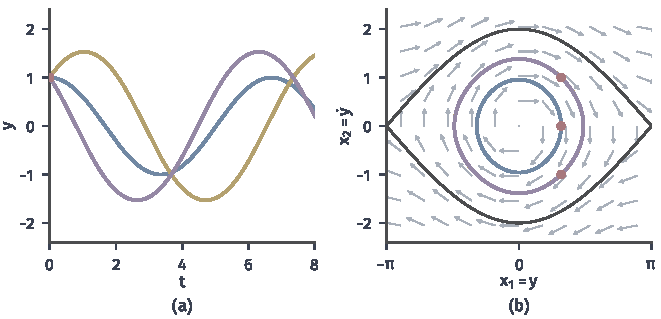
\includegraphics[width=112mm]{figures/06-differential-equations/01-ordinary-differential-equations/matplotlib/ivp-pendulum-state/figure.pdf}
 \caption{单摆$\ddot{y}=-\sin y$。三个初值都有$y(0)=1$，初始角速度为$0$（蓝）、$1$（黄）、$-1$（紫）。(a)角度随时间的变化。(b)相平面上的轨道：灰色箭头是右端的方向（长度已归一化），红点是初始状态，黄色和紫色的初始状态在同一条闭轨上。深灰色曲线$x_2=\pm 2\cos(x_1/2)$分开来回摆动与绕轴翻转两种运动。}
 \label{fig:ivp-pendulum-state}
\end{BookInlineFigure}

把$(x_1,x_2)$当作平面坐标，就得到图~\ref{fig:ivp-pendulum-state}(b)这样的\term{相平面}（phase plane）。每一点画一个箭头，表示状态在那一点的运动方向；解走过的路径称为\term{轨道}（orbit）。时间不再是坐标轴，而是沿轨道前进的快慢。这和方向场的区别在于：方向场的横轴是时间，所以一条解是从左往右的曲线；相平面没有时间轴，解可以绕回来。

相平面上的闭轨有一个可以手算的来源。定义$E=x_2^2/2+1-\cos x_1$，沿解求导，并用式~\eqref{eq:ivp-pendulum-system}代入：
\[
 \dot{E}=x_2\dot{x}_2+\sin x_1\,\dot{x}_1
 =x_2(-\sin x_1)+\sin x_1\,x_2=0.
\]
所以$E$沿解不变，解留在$E$的等值线上。三个初值的$E$分别是
\[
 E(1,0)=1-\cos 1\approx 0.460,\qquad E(1,\pm 1)=1.5-\cos 1\approx 0.960.
\]
后两个数相同，所以图中黄色与紫色的初值落在同一条闭轨上，只是位置不同。深灰色曲线对应$E=2$，也就是摆恰好能走到最高点的能量。

\paragraph{高阶方程化为一阶系统}
同样的做法适用于任意阶数。设标量未知函数$y$满足$m$阶方程
\begin{equation}
 y^{(m)}=h\bigl(t,y,\dot{y},\ldots,y^{(m-1)}\bigr).
 \label{eq:ivp-high-order}
\end{equation}
下一瞬间要知道的是$y$及其直到$m-1$阶的导数，所以令$x_j=y^{(j-1)}$，$j=1,\ldots,m$。这些量之间的关系如图~\ref{fig:ivp-state-chain}所示：前面每个分量的导数恰好是下一个分量，只有最后一个分量的导数由$h$决定。

\begin{BookInlineFigure}
 \centering
 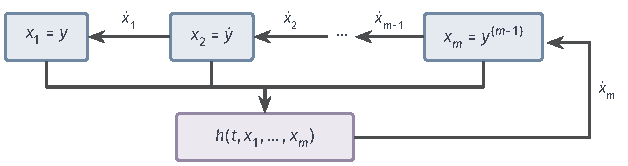
\includegraphics[width=106mm]{figures/06-differential-equations/01-ordinary-differential-equations/tikz/ivp-state-chain/figure.pdf}
 \caption{$m$阶方程的状态链。蓝框是状态的分量，水平箭头表示前一分量的导数等于后一分量，紫框由全部分量和时间算出最后一个分量的导数$\dot{x}_m$。}
 \label{fig:ivp-state-chain}
\end{BookInlineFigure}

\begin{lemma}[降阶]
 \label{lem:ivp-order-reduction}
 设$h$在$T\times\bm{D}$上有定义，$\bm{D}\subseteq\mathbb{R}^{m}$是开集，$I\subseteq T$是区间。函数$y:I\to\mathbb{R}$在$I$上$m$次可微且满足式~\eqref{eq:ivp-high-order}，并使$(y,\dot{y},\ldots,y^{(m-1)})$取值于$\bm{D}$，当且仅当
 \begin{equation}
 \bm{x}=\bigl(y,\dot{y},\ldots,y^{(m-1)}\bigr)
 \label{eq:ivp-reduction-state}
 \end{equation}
 在$I$上可微，取值于$\bm{D}$，并满足一阶系统$\dot{x}_j=x_{j+1}$（$j<m$），$\dot{x}_m=h(t,x_1,\ldots,x_m)$。
\end{lemma}

\begin{proof}
 若$y$满足式~\eqref{eq:ivp-high-order}，按定义~\eqref{eq:ivp-reduction-state}逐分量求导，前$m-1$个分量给出$\dot{x}_j=y^{(j)}=x_{j+1}$，最后一个分量给出
 \[
 \dot{x}_m=y^{(m)}=h(t,y,\ldots,y^{(m-1)})=h(t,x_1,\ldots,x_m).
 \]
 反过来，设一阶系统有可微解$\bm{x}$，令$y=x_1$。由$\dot{x}_1=x_2$，$y$可微且$\dot{y}=x_2$。$x_2$可微，所以$y$二次可微且$\ddot{y}=x_3$。依次进行到$x_m$，得到$y^{(m-1)}=x_m$，而$x_m$可微，于是$y$是$m$次可微的，并且$y^{(m)}=\dot{x}_m=h(t,y,\ldots,y^{(m-1)})$。
\end{proof}

相应的初值必须同时给出$y(t_0),\dot{y}(t_0),\ldots,y^{(m-1)}(t_0)$这$m$个数。$m$阶方程需要$m$个初始条件，道理就在这里。

下面用一个二阶方程走一遍。设
\[
 \ddot{y}+3\dot{y}+2y=\cos t,\qquad y(0)=1,\quad\dot{y}(0)=0.
\]
令$x_1=y$，$x_2=\dot{y}$，把二阶导数解出来，$\ddot{y}=\cos t-3\dot{y}-2y$，得到
\[
 \dot{\bm{x}}=\begin{pmatrix}0&1\\-2&-3\end{pmatrix}\bm{x}+\begin{pmatrix}0\\\cos t\end{pmatrix},\qquad
 \bm{x}(0)=\begin{pmatrix}1\\0\end{pmatrix}.
\]
这个系统的矩阵形式和解法由第~\ref{chap:linear-differential-systems}章给出。

\paragraph{状态、时间与外部输入}
上面的方程右端显含$\cos t$，它不是状态的一部分，而是外部施加的作用。给单摆加上阻力和一个随时间变化的驱动力矩$g(t)$，方程变成$\ddot{y}=-\sin y-c\dot{y}+g(t)$，其中$c\geq 0$是阻尼系数，状态方程是
\[
 \dot{x}_1=x_2,\qquad\dot{x}_2=-\sin x_1-cx_2+g(t).
\]
这里出现了三种不同地位的量：状态$(x_1,x_2)$由方程决定；驱动力矩$g$事先给定，不受状态影响；$c$是整段时间不变的常数。一般写法是图~\ref{fig:ivp-state-input-blocks}中的
\begin{equation}
 \dot{\bm{x}}=\bm{h}\bigl(\bm{x},\bm{g}(t),\bm{\theta}\bigr),
 \label{eq:ivp-input-system}
\end{equation}
其中$\bm{g}(t)$称为\term{外部输入}（external input），$\bm{\theta}$称为参数。

\begin{BookInlineFigure}
 \centering
 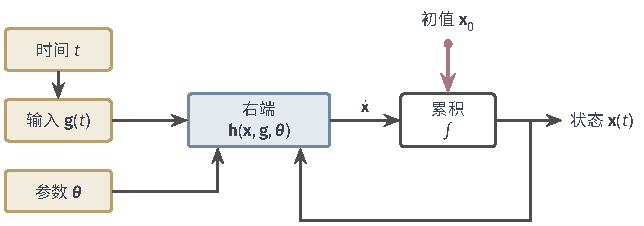
\includegraphics[width=109mm]{figures/06-differential-equations/01-ordinary-differential-equations/tikz/ivp-state-input-blocks/figure.pdf}
 \caption{状态方程的信息流。时间先决定输入，输入与参数同当前状态一起进入右端，得到变化率，再累积成状态，初值给累积的起点。状态沿反馈回路影响自己的变化率。}
 \label{fig:ivp-state-input-blocks}
\end{BookInlineFigure}

一旦$\bm{g}$和$\bm{\theta}$选定，就可以把它们代入右端，得到
\[
 \bm{f}(t,\bm{x})=\bm{h}\bigl(\bm{x},\bm{g}(t),\bm{\theta}\bigr),
\]
式~\eqref{eq:ivp-input-system}于是成为定义~\ref{def:ivp-ivp}的形式。时间$t$通过输入进入右端，所以$\bm{f}$显含时间。下面的表说明四种量的区别。

\begin{BookInlineTable}
 \centering
 \caption{初值问题中四种量的角色}
 \label{tab:ivp-roles}
 \begin{tabular}{lll}
 \toprule
 量 & 由谁决定 & 例子 \\
 \midrule
 时间$t$ & 自变量 & 钟面读数 \\
 状态$\bm{x}(t)$ & 由方程和初值决定 & 角度与角速度 \\
 外部输入$\bm{g}(t)$ & 事先给定的时间函数 & 驱动力矩 \\
 参数$\bm{\theta}$ & 事先给定的常数 & 阻尼系数$c$ \\
 \bottomrule
 \end{tabular}
\end{BookInlineTable}

分界并不是绝对的，要看问题怎么提。若力矩由当前角度算出，例如$g=-\beta x_1$，它就不再是事先给定的时间函数，而成了状态的函数，应当并入右端。

\paragraph{自治方程}
右端不显含时间的方程称为\term{自治方程}（autonomous equation），写作$\dot{\bm{x}}=\bm{f}(\bm{x})$，此时取$T=\mathbb{R}$；否则称为\term{非自治方程}（non-autonomous equation）。指数增长、饱和增长、冷却和无驱动的单摆都是自治的，$\dot{x}=\cos t$是非自治的。

自治意味着规律不随时间改变：今天和明天从同一状态出发，后面的故事相同，只是整体错开一段时间。

\begin{lemma}[自治方程的时间平移]
 \label{lem:ivp-time-shift}
 设$\bm{x}:I\to\bm{D}$满足$\dot{\bm{x}}=\bm{f}(\bm{x})$，$\tau\in\mathbb{R}$。则曲线$\tilde{\bm{x}}(t)=\bm{x}(t-\tau)$在平移后的区间$I+\tau$上也满足同一方程。
\end{lemma}

\begin{proof}
 由链式法则，$\dot{\tilde{\bm{x}}}(t)=\dot{\bm{x}}(t-\tau)$。再用方程在时刻$t-\tau$成立，得到
 \[
 \dot{\tilde{\bm{x}}}(t)=\bm{f}\bigl(\bm{x}(t-\tau)\bigr)=\bm{f}\bigl(\tilde{\bm{x}}(t)\bigr).
 \]
\end{proof}

图~\ref{fig:ivp-time-shift}对比了平移的结果，平移量都是$\tau=1.5$。(a)中方向场沿水平方向不变，黄线是蓝线向右平移的结果，依然处处与线段相切。(b)中方程是$\dot{x}=\cos t$，解$x=\sin t$平移后是$\sin(t-1.5)$，它的导数$\cos(t-1.5)$不等于右端$\cos t$，黄线穿过方向场的线段。

\begin{BookInlineFigure}
 \centering
 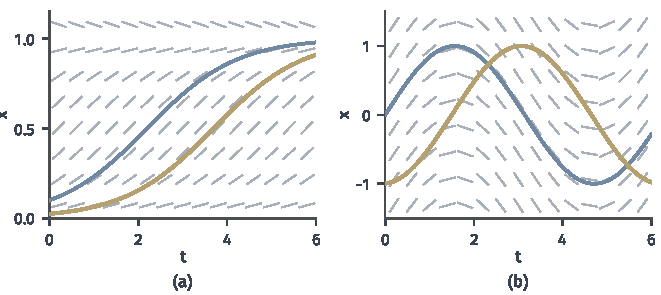
\includegraphics[width=112mm]{figures/06-differential-equations/01-ordinary-differential-equations/matplotlib/ivp-time-shift/figure.pdf}
 \caption{时间平移。蓝线是解，黄线是蓝线向右平移$1.5$的结果。(a)自治方程$\dot{x}=x(1-x)$：方向场沿时间方向不变，平移后仍是解。(b)非自治方程$\dot{x}=\cos t$：方向场随$t$变化，平移后不再与线段相切。}
 \label{fig:ivp-time-shift}
\end{BookInlineFigure}

\paragraph{用扩充状态消去显含时间}
非自治方程可以改写成自治方程，做法是把时间也当作一个状态分量。引入新分量$s$，规定$\dot{s}=1$，$s(t_0)=t_0$。扩充后的状态$\bm{z}=(\bm{x},s)\in\mathbb{R}^{n+1}$满足
\begin{equation}
 \dot{\bm{z}}=\bm{F}(\bm{z})=\begin{pmatrix}\bm{f}(s,\bm{x})\\1\end{pmatrix},\qquad
 \bm{z}(t_0)=\begin{pmatrix}\bm{x}_0\\t_0\end{pmatrix}.
 \label{eq:ivp-extended-state}
\end{equation}
这个系统的右端不显含$t$。由$\dot{s}=1$和初值，$s(t)=t_0+(t-t_0)=t$，所以$\bm{f}(s,\bm{x})$恰好就是$\bm{f}(t,\bm{x})$，式~\eqref{eq:ivp-extended-state}的前$n$个分量与原方程相同。反过来，原方程的解$\bm{x}$连同$s(t)=t$就是式~\eqref{eq:ivp-extended-state}的解。两个问题的解一一对应。

这个改写解释了状态的含义为什么要包括时间。取受迫振子$\ddot{y}+y=\cos 3t$，初值$y(0)=0.175$，$\dot{y}(0)=0.2$，解是$y(t)=0.3\cos t+0.2\sin t-\tfrac{1}{8}\cos 3t$。在$(x_1,x_2)=(y,\dot{y})$平面上，这条轨线在$t\approx 2.335$和$t\approx 3.027$经过同一点$(-0.157,-0.107)$，而两个时刻的右端分别约为
\[
 (-0.107,\ 0.908),\qquad(-0.107,\ -0.784).
\]
方向不同，说明只看$(x_1,x_2)$不足以决定下一瞬间的变化。图~\ref{fig:ivp-extended-lift}(b)把时间$s$加为第三个坐标，这两个时刻分到了不同的高度，交点随之消失。

\begin{BookInlineFigure}
 \centering
 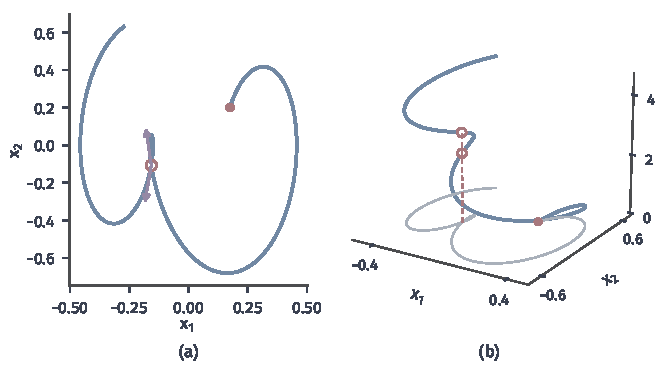
\includegraphics[width=112mm]{figures/06-differential-equations/01-ordinary-differential-equations/matplotlib/ivp-extended-lift/figure.pdf}
 \caption{受迫振子$\ddot{y}+y=\cos 3t$的轨线，$0\leq t\leq 4.6$。(a)在$(x_1,x_2)$平面上自交于空心点，紫色箭头是两个时刻右端的方向，红点是初值。(b)加入坐标$s=t$后，蓝线的两个对应点高度不同，灰线是它在底面上的投影。}
 \label{fig:ivp-extended-lift}
\end{BookInlineFigure}

改写是有代价的。维数增加一维；$\dot{s}=1$永不为零，所以扩充系统没有不动的状态；时间对右端的影响变成了状态对右端的影响，若$\bm{f}$对时间只有很差的正则性，$\bm{F}$对状态分量$s$的正则性也一样差。第~\ref{sec:ivp-measurable}节会看到这一点的后果。
